% master.tex : master-fil for projektet
% ------------------------------------------------------------------------------
% Dette er hovedfilen for projektet, hvori indhold fra alle input-filer (tekst,
% billeder, litteraturdatabaser, osv.) samles

% Dokumenttypen 'book' er valgt pga. dens mange fleksible indstillinger
% Se https://tex.stackexchange.com/a/36989/118167
\documentclass[11pt,a4paper,twoside,openright,danish]{book}

% Variabler, som bruges til automatisk at indsætte titel, forfattere, osv. på
% forsiden og titelbladet.
\def \projecttitle       {Optimering af gaslager}
\def \projectsubtitle    {Diskret optimering}
\def \projecttheme       {Optimering af gaslager}
\def \projectdegree      {Matematik-Økonomi}  % eller Matematik-Økonomi/Teknologi
\def \projectperiod      {Efterårssemesteret 2020}
\def \projectnumber      {P1}
\def \projectgroup       {B350}
\def \projectauthors     {
  Beate Marcussen\\
  Marcus Søndergaard Aaskoven\\
  Mathias Graversen\\
  Mattias Adam Arvidsson\\
  Vennan Vithiyatharan
  % ...
}
\def \projectsupervisors {
  Janus Valberg-Madsen\\
  % ...
}

% Preamblet indeholder alle de indstillinger og makroer, som skal indsættes for
% hovedindholdet, og i denne skabelon samles det i filen aaumath.sty, som
% definerer en pakke, der kan indlæses med \usepackage.
\usepackage{aaumath}
\usepackage{graphicx}
% Dokumentets indhold indsættes mellem \begin- og \end-makroerne for
% 'document'-blokken
\usepackage{amsthm}
\theoremstyle{definition}
\newtheorem{definition}
{Definition}[section]

\begin{document}

% Dokumentets 'front matter' tælles ikke med ifm. antal sider og nummereres med
% romerske tal. Herunder hører f.eks. forsiden, titelbladet, forordet og
% indholdsfortegnelsen.
\frontmatter
% incl/misc/frontpage.tex : rapportens forside
% ------------------------------------------------------------------------------


\backgroundsetup{
  scale = 1,
  angle=0,
  opacity=1,
  contents = {
    
\includegraphics[width=\paperwidth,height=\paperheight]{fig/img/aau/waves.pdf}
  }
}
\BgThispage
\pdfbookmark[0]{Forside}{forside}
\begin{titlepage}
  \centering
  \phantom{}
  \vspace{2cm}

  % AAU-segl
  \begin{minipage}[c]{0.2\paperwidth}
    \centering
    \makebox[0pt]{
      % fig/tikz/aau-badge.tex : AAU-logo til forsiden
% ------------------------------------------------------------------------------

\begin{tikzpicture}
  % Tegn hvid cirkel og tilføj det gennemsigtige, blå logo ovenpå
  \node[circle,color=white,fill=white,minimum size=1.175\textwidth] at (0,0) {};
  \node at (0,0) {
\includegraphics[width=\textwidth]{fig/img/aau/logo-circle.pdf}};
\end{tikzpicture}

    }
  \end{minipage}

  % Hovedindhold
  \vspace{4cm}
  {\fontfamily{bch}\selectfont
    \fboxsep0pt\colorbox{white}{
      \begin{minipage}{\textwidth}
        \centering
        \color{AAUblue1}

        \vspace{2em}
        {\Huge\bfseries\projecttitle}

        {\Large\bfseries\projectsubtitle}

        \bigskip
        \parbox{\textwidth}{\centering\large\projectauthors}

        \bigskip
        {\bfseries\large{\projectnumber}-Projekt, Gruppe \projectgroup, \projectdegree}
        \vspace{2em}
      \end{minipage}
    }
  }

\end{titlepage}

% incl/misc/titlepage.tex : rapportens titelblad
% ------------------------------------------------------------------------------
% Titelbladet genereres af makroen \aautitlepage, som er defineret i
% /incl/pre/ext/aautitlepage.sty


\pdfbookmark[0]{Titelblad}{titelblad}
\aautitlepage{
  \projectinfo{
    \projecttitle
  }{
    \projecttheme
  }{
    \projectperiod
  }{
    Gruppe \projectgroup
  }{
    \parbox[t]{\textwidth}{\projectauthors}
  }{
    \parbox[t]{\textwidth}{\projectsupervisors}
  }{
    \today
  }
}{
  \textbf{Institut for Matematiske Fag}\\
  Skjernvej 4A\\
  DK-9220 Aalborg Ø\\
  \href{http://math.aau.dk}{http://math.aau.dk}
}{
  % incl/misc/abstract.tex : projektets abstract 

This study investigates how algorithms and graph theory can help with the optimization of profit from a gas storage, over the course of a given period of time, by buying and selling gas units. 

In order to give clarification of the calculations and methods used in this study, the essential and relevant graph theory, and theory of algorithms will therefore be explained.
During this study it was found that Dijkstra's algorithm was very useful for solving shortest path problems in graphs. This study implements Dijkstra's algorithm in Python 3 in order to find the longest path through a graph. This can be done by finding the shortest path through the inverted non-negative graph. This path will be the path that yields the greatest profit. In addition, this path is the one that will give us the most optimal trading strategy.

The greatest profit in the original problem is 252.73€, and in the extended problem, it is 188.27€. From this, it can be concluded that the extensions that have been made, significantly reduce the profit. This is mainly due to the fluctuating limits of inventory, and the limits of buying and selling per month, as they affect the profit over the course of several months, compared to the penalty factor which only affects the last two months.

}

\tableofcontents

% Dokumentets 'main matter' (hovedindhold) er der, hvor det meste indhold skal
% sættes ind. Sider og overskrifter er nummererede med arabiske tal.
\mainmatter

\chapter{Forord}
Følgende projekt er udarbejdet af gruppe B350 bestående af fem stud.scient.oeconer på 1. semester på Aalborg Universitet. Projektet er skrevet i efteråret 2020 og beskæftiger sig med diskret matematik herunder optimering af et gaslager som basisproblem. Diskret matematik indgår i studiets læreplan og er derfor et relevant emne til projektskrivning. Projektet er skrevet i \LaTeX \ og delt med Git via GitAhead.
%Vi vil som gruppe rette en stor tak til vores vejleder Janus Valberg-Madsen for godt samarbejde gennem projektforløbet samt gode råd og rettelser.






%Eksempel på hvordan sætninger, definitioner mm. kan formateres. En mere effektiv løsning ville være at foretrække, men det kan bruges i mangel af bedre. (Hvor mørk baggrundsfarven er, ændres ved at ændre tallet efter udråbstegnet.

%\begin{mdframed}[linewidth=2pt, topline=false, rightline=false, bottomline=false, backgroundcolor=gray!50]
%\begin{thm}
%Tilfældig sætning
%\end{thm}
%\end{mdframed}
%
%\begin{mdframed}[style=MyStylethm]
%\begin{thm}
%Tilfældig sætning
%\end{thm}
%\end{mdframed}
%
%\begin{thm}
%Tilfældig sætning
%\end{thm}
%
%\begin{defn}[Definition]
%Tilfældig definition
%\end{defn}
%
%\begin{exmp}
%Tilfældigt eksempel
%\end{exmp}
%
%\begin{lem}
%Tilfældigt lemma
%\end{lem}
%
%\begin{prop}[Proposition]
%Tilfældig proposition
%\end{prop}
%
%\begin{cor}
%Tilfældigt Korollar
%\end{cor}
\chapter{Indledning}

\chapter{Algoritmer} \label{kap.algo}
Når man står med et problem inden for diskret matematik, er det første, man skal gøre at finde en model, der kan sætte problemet i matematisk kontekst. Denne model skal bestå af diskrete strukturer såsom funktioner, følger eller grafer, som vi omtalte i tidligere afsnit. Når man har opstillet en passende model til at løse problemet, skal man finde en metode, som kan løse det med denne model. Denne model skal helst tilpasses, så den kan løse det generelle problem. Det vil sige alle probemer af den type og form. Metoden skal bestå af en række trin, som slutteligt vil give resultatet. Disse trin kaldes en \emph{algoritme}. 
\begin{defn}
[Algoritmer] En algoritme er en begrænset mængde af præcist definerede instruktioner, der viser, hvordan et problem løses, eller hvordan en beregning udføres. 
\end{defn}
I følgende afnsit vil vi skrive alle algoritmer i pseudokode, som er en forsimplet form for programmeringssprog. Pseudokode kan ikke direkte implementeres i nogen programmer, da det ikke har en bestemt syntaks. Grunden til at vi skriver algoritmerne i pseudokode, er, at det er nemt at omskrive til forskellige andre programmeringssprog.


\section{Algoritmetyper}
Der findes mange typer algoritmer, som løser mange forskellige problemer. Vi vil i det følgende se på forskellige typer af algoritmer.
\subsection{Søgealgoritmer}
\emph{Søgealgoritmer} bruges til at løse problemer, hvor man vil finde et element, $x$, i en liste $(a_{1}, a_{2}, \dotsc, a_{n})$, eller konkludere, at $x$ ikke er i listen. Her vil løsningen være $i$, hvis $x=a_{i}$. Det er altså indekset, der er løsningen. Søgealgoritmer kan igen opdeles i forskellige typer bl.a. \emph{den lineære søgning} og \emph{den binære søgning}. Ved den lineære søgning starter man med $a_1$ og ser, om $x=a_{1}$. Hvis dette er tilfældet, er $a_{1}$'s indeks svaret, men hvis $x \neq a_{1}$, fortsætter man til $a_{2}$ og så $a_{3}$. Sådan fortsætter man, indtil man finder et element i listen, der er lig $x$, og så vil løsningen være dette elements indeks. \autoref{alg:lineaer} illustrerer et eksempel på en lineær søgealgoritme:

\begin{algorithm}[H] 
\caption{Den lineære søgealgoritme}
\begin{algorithmic}[1]

\Procedure{lineær søgning($x$: heltal, $a_{1},a_{2},\dotsc,a_{n}$: Heltal i listen)}{}
    \State $i:=1$
    \While{$i \leq n$ \textbf{and} $x \neq a_{i}$}
        \State $i:=i+1$
    \EndWhile
    \If{$i \leq n$} 
    \State \textbf{return} $lokation:=i$
    \Else
    \State \textbf{return} $lokation:=0$
    \EndIf
  \label{roy's loop}
\EndProcedure

\end{algorithmic}
\label{alg:lineaer}
\end{algorithm}


Modsat den lineære søgning kan den binære søgning kun bruges, når en liste er \emph{ordnet}. Det vil sige, hvis listen fx er voksende, aftagende eller alfabetisk, altså $(a_{1}<a_{2}<\dotsb<a_{n})$. Den binære søgealgoritme finder nu midten af listen, $a_{m}$, hvor $m=\left \lfloor \frac{n+1}{2} \right \rfloor$. $\lfloor \rfloor$ er flooroperatoren der runder ned til første heltal. Vi ser nu, hvilken side det, vi søger, er på. Hvis $a_{m}<x$, tager vi halvdelen af listen, der er større end $a_{m}$ dvs: $(a_{m+1}, a_{m+2},\dotsc,a_{n})$. Ellers tager vi halvdelen mindre end og lig $a_{m}$: $(a_{1}, a_{2},\dotsc,a_{m})$. Når vi har vurderet hvilken side af midten, den værdi, vi søger, er på, deles denne halvdel på midten, hvorefter man igen skal vurdere, hvilken side man skal arbejde videre med. Dette fortsættes, indtil tallet er fundet. Den binære søgealgoritme er illustreret i \autoref{alg:binaer}.

\begin{algorithm}[H]
\caption{Den binære søgealgoritme}
\begin{algorithmic}[1]

\Procedure{binær søgning($x$: heltal, $a_{1},a_{2},\dotsc,a_{n}$: Voksende heltal i listen)}{}
    \State $i:=1$, \{$i$ er venstre endepunkt i søgeintervallet\}
    \State $j:=n$, \{$j$ er højre endepunkt i søgeintervallet\}
    \While{$i<j$}
        \State $m=\lfloor (i+j)/2 \rfloor$
    		\If{$x>a_{m}$}
    		\State $i:=m+1$
    		\Else
    		\State $j:=m$
    		\EndIf    
    \EndWhile
    \If {$x=a_{i}$}
    	\State \textbf{return} $lokation:=i$
    \Else
    	\State \textbf{return} $lokation:=0$
    \EndIf
  \label{roy's loop}
\EndProcedure

\end{algorithmic}
\label{alg:binaer}
\end{algorithm}

\subsection{Sorteringsalgoritmer} \label{kap:sortering}
Når vi arbejder med \emph{sorteringsalgoritmer}, er det, fordi vi ønsker at sortere en liste, således at den inddeles i fx voksende rækkefølge eller alfabetisk orden. Ligesom ved søgealgoritmerne er der flere forskellige sorteringsalgoritmer. Eksempler på disse er \emph{bubblesortering} og \emph{indskudssortering}. Bubblesortering er en af de simpleste sorteringsalgoritmer, men den er ikke så effektiv. Vi vil komme ind på algoritmers effektivitet i \autoref{kap:kompleksitet}. Den sammenligner tilstødende værdier i en liste og bytter om på dem, hvis rækkefølgen ikke er korrekt.

\begin{algorithm}[H]
\caption{Bubblesorteringsalgoritmen}
\begin{algorithmic}[1]

\Procedure{bubblesortering($a_{1},a_{2},\dotsc,a_{n}$: Reelle tal hvor $n \geq 2$)}{}
\EndProcedure
\For {$i:=1$ \textbf{to} $n-1$}
    	\For {$j:=1$ \textbf{to} $n-i$}
    		\If {$a_{j}>a_{j+1}$}
    			\State Ombyt $a_{j}$ og $a_{j+1}$ 	
\EndIf
\EndFor
\EndFor
\State $a_{1},a_{2},\dotsc,a_{n}$ er i voksende rækkefølge. 

\end{algorithmic}
\end{algorithm}

\begin{exmp}
Vi ser på en liste, $(3,4,2,5,1)$, som vi vil arrangere således, at den er i rækkefølge med stigende værdi. Algoritmen gentages fire gange, da listen har længden $n=5$, og algoritmen skal køre $n-1$ gange. 
\begin{align*}
	\text{Første gentagelse:} \qquad \qquad \qquad \quad \text{Anden 			gentagelse:} \qquad \qquad \qquad \quad \text{Tredje gentagelse:} 			\qquad \qquad \qquad \quad \\
	(\textbf{3,4},2,5,1) \rightarrow (\textbf{3,4},2,5,1) \qquad \qquad 		(\textbf{3,2},4,1,5) \rightarrow (\textbf{2,3},4,1,5) \qquad \qquad 		(\textbf{2,3},1,4,5) \rightarrow (\textbf{2,3},1,4,5) \qquad \qquad 		\\
	(3,\textbf{4,2},5,1) \rightarrow (3,\textbf{2,4},5,1) \qquad \qquad     	(2,\textbf{3,1},4,5) \rightarrow (2,\textbf{1,3},4,5) \qquad \qquad   	(2,\textbf{3,1},4,5) \rightarrow (2,\textbf{1,3},4,5) \qquad \qquad 		\\
	(3,2,\textbf{4,5},1) \rightarrow (3,2,\textbf{4,5},1) \qquad \qquad 		(2,1,\textbf{3,4},5) \rightarrow (2,1,\textbf{3,4},5) \qquad \qquad  	\qquad \qquad \qquad \qquad \qquad \qquad \qquad \quad \ \ \\
	(3,2,4,\textbf{5,1}) \rightarrow (3,2,4,\textbf{1,5}) \qquad \qquad 		\qquad \qquad \qquad \qquad \qquad \qquad \qquad \quad \ \  \qquad 			\qquad \qquad \qquad \qquad \qquad \qquad \quad \ \
\end{align*}

\begin{flushleft}
Fjerde gentagelse:
\\
$(\textbf{2,1},3,4,5) \rightarrow (\textbf{1,2},3,4,5)$
\end{flushleft}

Efter første gentagelse har algoitmen placeres det største tal bagerst i listen, efter anden gentagelse har algoritmen placeret det næst største tal på næst sidste plads i listen. Således fortsætter algoritmen indtil listen er i korrekt rækkefølge.

\end{exmp}

Indskudssortering er på samme måde som bubblesortering simpel og til tider ineffektiv. For denne algoritme gælder det, at man starter med den anden værdi i listen, som sammenlignes med den første værdi. Disse to sorteres nu efter størrelse. Den tredje værdi i listen sammenlignes derefter med den første. Hvis den er større, sammenlignes den med den anden værdi i listen, og på den måde sorteres hele rækken, så de til sidst står i rækkefølge.

\begin{algorithm}[H]
\caption{Indskudssorteringsalgoritmen}
\begin{algorithmic}[1]

\Procedure{indskudssortering($a_{1},a_{2},\dotsc,a_{n}$: Reelle tal hvor $n \geq 2$)}{}
\EndProcedure
\For {$j:=2$ \textbf{to} $n$}
	\State $i:=1$
    	\While {$a_{j}>a_{i}$}
    		\State $i:=i+1$
    	\EndWhile
    	\State $m:=a_{j}$
    	\For {$k:=0$ \textbf{to} $j-i-1$}
    		\State $a_{j-k}:=a_{j-k-1}$
    	\EndFor
    	\State $a_{i}:=m$
\EndFor
\State $a_{1},a_{2},\dotsc,a_{n}$ er i voksende rækkefølge. 

\end{algorithmic}
\end{algorithm}

\begin{exmp}
Vi ser igen på en liste, $(3,4,2,5,1)$, som vi gerne vil sortere i rækkefølge, således at de står med stigende værdi. Til at gøre dette, vil vi bruge indskudssorteringsalgoritmen. Illustrationen, som ses nedenfor, viser, at alle understregede tal står i korrekt rækkefølge. Tallet markeret med fed er det næste tal, som algoritmen skal placere i den korrekte liste.

\begin{figure}[H]
\label{fig:indskud}
	\begin{flushleft}
	$i=1: \ (\underline{3},\textbf{4},2,5,1) \rightarrow (\textbf{4}, \underline{3},2,5,1)\rightarrow (\underline{3,\textbf{4}},2,5,1)$ \\
	$i=2: \ (\underline{3,4},\textbf{2},5,1) \rightarrow (\underline{\textbf{2},3,4},5,1) $\\
	$i=3: \ (\underline{2,3,4},\textbf{5},1) \rightarrow (\textbf{5},\underline{2,3,4},1) \rightarrow (\underline{2}, \textbf{5},\underline{3,4},1) \rightarrow (\underline{2,3}, \textbf{5}, \underline{4},1) \rightarrow (\underline{2,3,4,\textbf{5}},1) $ \\
	$i=4: \ (\underline{2,3,4,5},\textbf{1}) \rightarrow (\underline{\textbf{1},2,3,4,5}) $\\
 	\end{flushleft}
\end{figure}

Vi kan se, at algoritmen starter med at sammenligne fire med tre. Den tjekker først, om fire er mindre end tre. Da det er større, og der ikke er flere tal i listen, placeres fire i slutningen af den korrekte liste. Den tjekker nu det tredje tal i listen og ser med det samme, at det er mindre end det første tal i den korrekte liste. Derfor placeres to på den første plads i den korrekte liste. Den sammenligner nu fem med alle tal i den korrekte liste og placerer fem efter det største tal, den er større end. Dette gør den med alle tallene i listen, og den har til sidst placeret alle tallene i listen i korrekt rækkefølge.


\end{exmp}
\subsection{Grådige algoritmer}
Når man arbejder med optimeringsproblemer, som handler om enten at minimere eller maksimere noget som fx at finde den længste eller korteste vej i en graf, kan man ofte bruge \emph{grådige algoritmer}.
En grådig algoritme vælger altid det \emph{lokalt optimale} valg og antager, at dette medfører en \emph{global optimal} løsning, altså den bedst mulige løsning. Det lokalt optimale valg findes ved at vælge den umiddelbart bedste løsning for hvert muligt trin.
I mange tilfælde vil dette lede til global optimering, men der kan også forekomme situationer, hvor algoritmen vil finde en suboptimal løsning. Ligegyldigt om algoritmen finder en optimal eller suboptimal løsning, kalder vi den en grådig algoritme.

\begin{exmp}
Det danske møntsystem har seks forskellige mønter med værdier på $0.5,\ 1,\ 2,\ 5,\ 10$ og $20$ kroner. Systemet er optimeret således, at man kan lave byttepenge vha. en grådig algoritme. Man kan altid finde den optimale løsning ved at tage så mange af de mest værdifulde mønter først og derefter tage så mange som muligt af de næst mest værdifulde mønter. Man fortsætter denne proces, indtil man har den ønskede mængde byttepenge.
\begin{algorithm} [H]
\caption{Grådig algoritme til byttepenge}
\begin{algorithmic}[1]

\Procedure{Byttepenge($c_1,c_2,\dotsc,c_r$: værdien af mønter, hvor $c_1>c_2>\dotsb >c_r;n:$ et positivt heltal)}{}
\EndProcedure
\For{$i:=1$ \textbf{to} $r$}
    \State $d_i:=0$ ($d_i$ tæller mængden af mønter med værdi $c_i$)
    \While{$n \geq c_i$}
    	\State $d_i := d_i+1$ (Mængden af mønter med værdi $c_i$ øges med en.)
    	\State $n := n-c_i$
\EndWhile
\EndFor
\State ($d_i$ er mængden af mønter med værdi $c_i$ for $i=1,2,\dotsc,r$)
\end{algorithmic}
\end{algorithm}
Denne algoritme vil altid vælge den optimale løsning i dette specifikke problem, der kan dog være problemer, hvis mønternes værdi ændrer sig. 
Hvis vi forestiller os, at vi har et møntsystem med udelukkende tre mønter af værdi $25$, $10$ og $1$ i kroner. Der opstilles nu et problem, hvor vi vil have $30$ kroner i byttepenge, da vil denne algoritme få en løsning, som bruger én mønt af værdi $25$ og fem mønter af værdi $1$. Dette er en suboptimal løsning, da man kunne have brugt tre mønter af værdi $10$.
Dette viser, at grådige algoritmer ikke altid finder den optimale løsning.
\end{exmp}

Grådige algoritmer bruges også i grafteori til fx at løse korteste eller længste vej-problemer. Her vælger algoritmen den lokalt optimale vej fra startknuden til en naboknude. En grådig algoritme ser nu bort fra alle andre muligheder som ikke bruger denne knude.

\begin{figure}[H]
\centering
	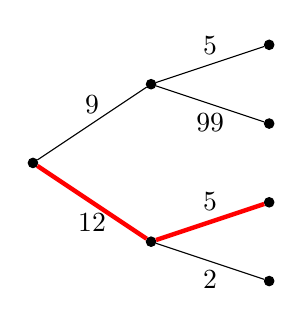
\begin{tikzpicture}

      \tikzset{enclosed/.style={draw, circle, inner sep=0pt, minimum size=.12cm, fill=black}}
% Vertices
      	\node[enclosed] (v1) at (0,2) {};
      	\node[enclosed] (v2) at (1.5,1) {};
    	\node[enclosed] (v3) at (1.5,3) {};
  	    \node[enclosed] (v4) at (3,0.5) {};
  	    \node[enclosed] (v5) at (3,1.5) {};
  	    \node[enclosed] (v6) at (3,3.5) {};
  	    \node[enclosed] (v7) at (3,2.5) {};    
%Edges
		\path (v1) edge[red, ultra thick] node[midway, below, black] {$12$} (v2);
		\path (v1) edge node[midway, above] {$9$} (v3);
		\path (v2) edge[red, ultra thick] node[midway, above, black] {$5$} (v5);
		\path (v2) edge node[midway, below] {$2$} (v4);
		\path (v3) edge node[midway, above] {$5$} (v6);
		\path (v3) edge node[midway, below] {$99$} (v7);


	\end{tikzpicture}
	\caption{Længste vej ifølge grådig algoritme.}
	\label{fig:greedy.eks}
\end{figure}

\autoref{fig:greedy.eks} et eksempel på en grådig algoritme, som har forsøgt at finde den længste mulige simple vej i en graf. Vi kan se, at algoritmen har valgt de lokalt optimale valg, men har ikke fundet den global optimale løsning. Det er tydeligt at se, at denne algoritme ikke er pålidelig nok til at løse sådanne problemer. Der findes dog nogle grådige algoritmer som er optimeret således de altid finder den globalt optimale løsning, så længe grafen overholde specifikke krav. Dette ser vi i \autoref{kap:dijkstras}


\section{Dijkstras algoritme}
I \ref{defn:min.vej} definerede vi distancen af den korteste vej i en vægtet graf. For at finde den korteste vej vil vi anvende \emph{Dijkstras algoritme}. Dijkstras algoritme kan bruges til at finde den korteste vej i en simpel, vægtet graf, hvori vægtene for alle kanter i grafen skal være ikke-negative. Algoritmen fungerer således, at den finder den korteste vej fra en startknude, $v_{1}$, til en endeknude, $v_{m}$, ved først at finde naboknuderne til $v_{1}$ og undersøge hvilken af disse, der har den mindste distanceværdi og altså er tættest på startknuden. Derefter tager den udgangspunkt i den naboknude, hvortil distanceværdien er mindst og fortsætter ad dennes vej, så længe denne vej har en mindre distanceværdi end en alternativ vej. Fremgangsmåden vil her illustreres ved hjælp af et eksempel, som tager udgangspunkt i \ref{kap:grafteori}.

\begin{exmp}
Betragt figur \ref{fig.dijkstraexmp}
\begin{figure}[H]
\centering
	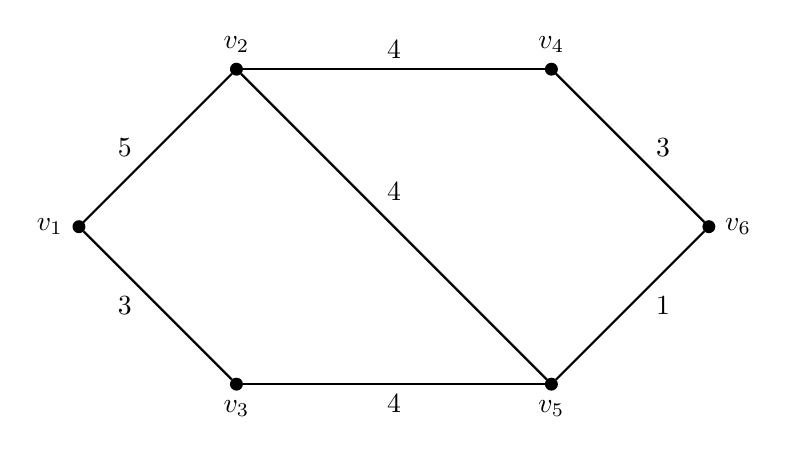
\begin{tikzpicture}

      \tikzset{enclosed/.style={draw, circle, inner sep=0pt, minimum size=.15cm, fill=black}}
%% Vertices
      	\node[enclosed, label={left: $v_1$}] (v1) at (0,2) {};
      	\node[enclosed, label={above: $v_2$}] (v2) at (2,4) {};
    	\node[enclosed, label={below: $v_3$}] (v3) at (2,0) {};
  	    \node[enclosed, label={above: $v_4$}] (v4) at (6,4) {};
     	\node[enclosed, label={below: $v_5$}] (v5) at (6,0) {};
     	\node[enclosed, label={right: $v_6$}] (v6) at (8,2) {};
%Edges
		\path [-, > = latex, thick] (v1) edge node[midway, left=2mm] {$ 5 $} (v2);
		\path [-, > = latex, thick] (v1) edge node[midway, left=2mm] {$ 3 $} (v3);
		\path [-, > = latex, thick] (v2) edge node[midway, above] {$ 4 $} (v4);
		\path [-, > = latex, thick] (v2) edge node[midway, above=2mm] {$ 4 $} (v5);
		\path [-, > = latex, thick] (v3) edge node[midway, below] {$ 4 $} (v5);
		\path [-, > = latex, thick] (v4) edge node[midway, right=2mm] {$ 3 $} (v6);
		\path [-, > = latex, thick] (v5) edge node[midway, right=2mm] {$ 1 $} (v6);

	\end{tikzpicture}
	\caption{Simpel, vægtet graf.}
	\label{fig.dijkstraexmp}
\end{figure}
I figur \ref{fig.dijkstraexmp} vil vi finde den korteste vej fra $v_{1}$ til $v_{6}$. Dijkstras algoritme vil gøre dette ved at finde den korteste vej fra startknuden, $v_{1}$, til hver knude, indtil den når endeknuden, $v_{6}$. Først vil den se, at startknuden har naboknuderne $v_{2}$ og $v_{3}$. Der er altså to veje fra startknuden, $P=(v_{1},v_{2})$ med distancen 5 og $P=(v_{1},v_{3})$ med distancen 3. Dermed er $v_{3}$ den knude, der er tættest på startknuden. Herefter er der igen to veje, $P=(v_{1},v_{2})$ med distancen 5 og $P=(v_{1},v_{3},v_{5})$ med distancen 7. Den første af disse vælges, da denne har den mindste distance, og $v_{2}$ er dermed knuden, som er næsttættest på startknuden. Nu er der tre forskellige veje, $P=(v_{1},v_{2}, v_{4})$ med distancen 9, $P=(v_{1},v_{2}, v_{5})$ med distancen 9 og $P=(v_{1},v_{3}, v_{5})$ med distancen 7. Den tredje vælges, og det er nu noteret, at den korteste vej fra $v_{1}$ til $v_{5}$ har distancen 7. Der er nu igen kun to mulige veje at vælge imellem, $P=(v_{1},v_{2}, v_{4})$ med distancen 9 og $P=(v_{1},v_{3}, v_{5}, v_{6})$ med distancen 8. $P=(v_{1},v_{2}, v_{5})$ er ikke længere en mulig vej, da vi allerede har fundet den korteste vej fra $v_{1}$ til $v_{5}$. Den anden vej har den mindste distance, og derfor vælger vi denne, og vi ved nu, at den korteste vej fra $v_{1}$ til $v_{6}$ er $P=(v_{1},v_{3}, v_{5}, v_{6})$ og har distancen 8.
\end{exmp}

Ovenstående eksempel er simpelt og kan hurtigt løses ved fx brute force metoden, men i større og mere komplicerede grafer er Dijkstras algoritme meget mere effektiv. For at skabe yderligere overblik over hvordan Dijkstras algoritme fungerer, vil vi her gå i dybden med dennes mere teoretiske del.
\begin{algorithm}[H]
\caption{Dijkstras algoritme}
\begin{algorithmic}[1]

\Procedure{dijkstra($G$: vægtet, sammenhængende, simpel graf med kun ikke-negative vægte)}{}
    \State \{$G$ {har knuderne $a = v_{1}, v_{2}, \dotsc, v_{m} = z$ og vægtene til kanterne $w(v_{i}, v_{j})$, hvor $w(v_{i}, v_{j}) = \infty$ hvis $v_{i}$ og $v_{j}$ ikke er naboer \}}
	\For {$i := 2$ \textbf{to} $m$}
		\State $L(v_{i}) := \infty$
	\EndFor
	\State $L(a) := 0$	
	\State $S := \emptyset$
	\State {\{distancen til hver knude initialiseres, så $a = 0$, og distancen til alle andre knuder er $\infty$, derudover er $S$ defineret som en tom mængde\}}
    \While{$z \notin S$}
        \State {$u :=$ en knude som ikke er i $S$ med $L(u)$ som minimum}
        \State $S := S \cup \{u\}$
        \For {alle $v \notin S$}
        	\If {$L(u) + w(u,v) < L(v)$} {$L(v) := L(u) + w(u,v)$}
        	\State \{dette tilføjer knuder til $S$ med minimal 			distance og opdaterer distancerne til
        	\State knuderne, som ikke er i $S$\}
        	\EndIf
    	\EndFor
    \EndWhile
    \State {\textbf{return} $L(z)$ \{$L(z) = \alpha(a,z)$\}} 
\EndProcedure

\end{algorithmic}
\label{alg:dijkstra}
\end{algorithm}
Det første, der sker, er, at startknuden noteres som $0$, og resten af knuderne noteres som $\infty$. Her betegnes den korteste vej som $\alpha_{k}(v_1,v_m)$, fra definition \ref{defn:min.vej}, hvor $k$ er antallet af \emph{iterationer} gennemført i algoritmen. Antallet af iterationer er det antal gange en løkke gennemkøres, altså hver gang vejen opdateres. Distancen af den korteste vej algoritmen finder fra startknuden til en given knude, noterer vi her ved $L$. $L_{0}(v_1)=0$ betyder altså, at vi har nul iterationer og dermed kun kender startknuden med distancen $0$. Derudover oprettes en mængde $S$, for hvilken det gælder, at $S = \emptyset$ når $k = 0$. Ved første iteration undersøges startknudens naboknuder, og man bestemmer, som i eksemplet ovenfor, hvilken distance er mindst. Dermed er startknudens nærmeste knude fundet, og denne tilføjes nu til mængden $S$. For hver iteration tilføjes et nyt element til mængden, og denne proces fortsætter, til algoritmen har fundet den korteste vej fra startknuden til endeknuden. Mængden, $S$, indeholder til sidst distancerne for den korteste vej fra startknuden til alle knuder i grafen. 

Ved brug af ovenstående metode kan vi illustrere løsningen til korteste vej-problemet fra \autoref{fig.dijkstraexmp} i en tabel.

\begin{table}[H]
\centering
\begin{tabular}{|c|c|c|c|c|c|c|}
\hline
$v$ & $v_1$ & $v_2$ & $v_3$ & $v_4$ & $v_5$ & $v_6$ \\ \hline
  & $\boldsymbol{0}$ &  $\infty$ & $\infty$  & $\infty$  &  $\infty$  &  $\infty$  \\  
 $v_1$ &  & $5_{v_1}$ & $\boldsymbol{3_{v_1}}$ & $\infty$ & $\infty$ & $\infty$ \\  
 $v_3$ &  & $\boldsymbol{5_{v_1}}$ &  & $\infty$ & $7_{v_3}$ & $\infty$ \\  
 $v_2$ &  &  &  & $9_{v_2}$ & $\boldsymbol{7_{v_3}}$ & $\infty$ \\
 $v_5$ &  &  &  & $9_{v_2}$ &  & $\boldsymbol{8_{v_5}}$   \\ \hline
\end{tabular}
\caption{Tabellarisk løsning til korteste vej i \autoref{fig.dijkstraexmp}.}
\label{tab:dijkstraexmp}
\end{table}

\begin{thm}[Dijkstras algoritme] \label{thm:dijkstra}
Dijkstras algoritme finder distancen af den korteste vej mellem to knuder, $v_1,v_m$, i en vægtet, sammenhængende og simpel graf sådan at $L(v_m)=\alpha(v_1,v_m)$. 
\end{thm}

\begin{proof}
Sætning \ref{thm:dijkstra} kan bevises ved induktion. Ved et induktionsbevis etablerer vi først et basisskridt, og dernæst opstiller vi en induktionshypotese. Basisskridtet består blot i, at vi undersøger distancen fra startknuden til startknuden, som selvfølgelig er 0, hvilket algoritmen også noterer. Vi har dermed $L(v_1)=0= \alpha(v_1,v_1)$, hvilket er sandt.
Vi opstiller nu vores induktionshypotese, hvor vi antager, at Sætning \ref{thm:dijkstra} er sand for $k$ iterationer. Det gælder altså at

\begin{equation}
L(v_m) = \alpha(v_1,v_m), \forall v \in S_k \textrm{ for vejen } P = (v_1, v_2, \dotsc, v_m).
\end{equation}
Vi sætter nu $v_{n}$ til at være den knude, der tilføjes til $S$ ved $S_{k+1}$. Vi vil nu vise, at det ligesom ved alle tidligere knuder i $S$ også gælder for $v_{n}$ at $L(v_n)=\alpha(v_1,v_n)$. Dette kan bevises ved modstrid. Vi starter med at antage, at der findes en kortere vej fra $v_1$ til $v_n$ end $L(v_n)$. Vi kalder denne nye vej $P_1$. For denne må det gælde at

\begin{equation}
dist(P_1)<L(v_n).
\end{equation}
$P_1$ starter i $S_k$ og forlader på et tidspunkt denne mængde for at komme til $v_n$, som ikke er i $S_k$. Vi lader $v_x,v_y$ være den første kant på vejen $P_1$, der forlader $S_k$. $P_x$ betegnes som delen af vejen $P_1$, som går fra $v_1$ til $v_x$. Så ved vi at

\begin{equation}
dist(P_x)+w(v_x,v_y) \leq dist(P_1).
\end{equation}
Eftersom $v_x$ er i $S_k$, ved vi som følge af induktionshypotesen, at den korteste vej fra $v_1$ til $v_x$ er $L(v_x)$. Dermed ved vi at $L(v_x) \leq dist(P_x)$ og

\begin{equation}
L(v_x) + w(v_x,v_y) \leq dist(P_1).
\end{equation}
$v_y$ er nabo til $v_x$, hvilket betyder at

\begin{equation}
L(v_y) \leq L(v_x) + w(v_x,v_y).
\end{equation}
Eftersom hverken $v_n$ eller $v_y$ er i $S_k$, og algoritmen oprindeligt valgte $v_n$ i den $k+1$'te iteration, må $v_n$ have den mindste distance af de to således at

\begin{equation}
L(v_n) \leq L(v_y).
\end{equation}
Dette resulterer dog i, at vi påstår, at $L(v_n) < L(v_n)$. Dette kan ikke lade sig gøre, og vi konkluderer derfor, at der ikke findes en tilfældig kortere vej, $P_1$. $L(v_n)=\alpha(v_1,v_n)$ må altså være sandt, og Dijkstra algoritme finder den korteste vej.
\end{proof}

\section{Kompleksitet} \label{kap:kompleksitet}
%side 250 ish
%table 1 side 247 i pdf.

Der findes to former for kompleksitet, men vi vælger at fokusere på tidskompleksitet. Den anden form for kompleksitet er pladskompleksitet. 
Der er tre former for tilfælde: bedste, værste og gennemsnitlige. 
I bedste tilfælde ser man på det laveste antal trin for en inputstørrelse, $n$. I værste ser man på det højeste og i gennemsnittet, det gennemsnitlige. 
\emph{Bedste tilfælde} beskriver algoritmen under optimale forhold, i en lineær søgealgoritme vil dette altså være, at elementet der søges efter, er det første element i listen. 
Oftere ser man på enten \emph{værste tilfælde} eller \emph{gennemsnitlige tilfælde}. 
Det gennemsnitlige tilfælde vil give et rigtigt godt overblik over hvor god algoritmen er, dog er det meget svært at bestemme hvad et gennemsnitligt input er, da det er svært at bestemme nogle parametre at vælge ud fra. 
Det værste tilfælde giver et godt overblik over hvor lang tid det kan tage. Ved man at algoritmen er lineær i værste tilfælde, vil man kunne løse den i rimelig tid for alle størrelser $n$.
De forskellige resultater i vores analyse af algoritmerne, kan deles op i kategorier, de mest gængse er: $\log n$, $\sqrt{n}$, $n$, $n^x$, $x^n$ og $n!$, men det kan også være en kombination af disse, som $n!n$, $n\log n$ eller lignende.
For at beskrive disse algoritmer i fx værste tilfælde, vil man bruge operatorerne \emph{store-O}, \emph{store-Omega} og \emph{Theta}. Man vil her fokusere på \emph{asymptotiske $n$-værdier}, altså ved rigtigt store værdier for $n$, da man i nogle tilfælde vil have en algoritme der er langsommere end den øvre bindende funktion ved små $n$, men ved større, som fx over 10.000, er hurtigere.

\subsection{Store-$O$}
\begin{defn}
$f(n)= O(g(n))$ hvis og kun hvis $\exists$ positive konstanter $C$ og $n_o$ så at $|f(n)| \leq C |g(n)| \forall n \geq n_o$.
\end{defn}

Store-$O$ bliver brugt til at binde funktionen opadtil, begrænse den oppe fra. Man kan med garanti sige, at algoritmen tager store-$O$ tid eller mindre. 
\begin{exmp}
\begin{align*}
f(n)=& 13n+3 \\
13n+3 \leq& 20n \forall \ n \geq 1 \\
f(n) =& O(n).
\end{align*}
\end{exmp}
Man vil også kunne sige, at $f(n)$ er mindre end $n!$ eller en anden vilkårlig højere funktion $g(n)$, men da man altid vil vælge den mest begrænsende funktion, vil $n$ være det mest præcise. 

\subsection{Store-$\Omega$}
\begin{defn}
$f(n) = \Omega(g(n))$ hvis og kun hvis $\exists$ positive konstanter $C$ og $n_o$ så at $|f(n)| \geq C |g(n)| \forall n \geq n_o$.
\end{defn}
Store-Omega bruges, omvendt store-$O$, til at binde funktionen nedadtil, altså finde den nedre grænse for algoritmen, den vil mindst tage store-Omega tid i det givne tilfælde.
\begin{exmp}
\begin{align*}
f(n)=& 13n+3 \\
13n+3 \geq& n \forall \ n \geq 1 \\
f(n) =& \Omega(n).
\end{align*}
\end{exmp}

På samme måde som ved store-$O$-notationen, vil man her kunne vælge en vilkårlig mindre funktion, $logn$, $1$ med flere, men da man vil begrænse den så meget som muligt, vælger man den største funktion $g(n)$ hvor uligheden stadig er sand.
\subsection{Store-$\Theta$}
\begin{defn}
$f(n) = \Theta(g(x))$ hvis og kun hvis $\exists$ positive konstanter $C_1, C_2$ og $n_o$ så at $C_1|g(n)| \leq |f(n)| \leq C_2|g(n)| \forall n \geq n_o$.
\end{defn}
Når man har fundet den øvre og den nedre grænse, store-O og store-Omega, kan man finde Theta, den tætte bundne funktion,
\begin{exmp}
\begin{align*}
f(n)=& 13n+3 \\
\Omega(n) \leq& f(n) \leq O(n) \\
n \leq& 13n+3 \leq 10n \forall \ n \geq 1 \\
f(n) =& \Theta(n).
\end{align*}
\end{exmp}

I følgende afsnit tager vi udgangspunkt i to sorteringer, og ser hvordan de sammenligner sig på Store-$O$ i bedste og værste tilfælde.

\subsection{Kompleksitet af bubblesortering} \label{kap:kom_bubble}

For at finde kompleksiteten af bubblesortering, bruger vi store-$O$-notationen fra tidligere. 
Bubblesortering, som nævnt i \autoref{kap:sortering}, sammenligner to elementer fra listen, og flytter rundt på dem, hvis de står i forkert rækkefølge.
Vi starter med værste tilfælde. Her ser vi på en liste, $P$, der er sorteret i omvendt rækkefølge. $P = (5,4,3,2,1)$.
i første gennemgang sammenligner den 5 med 4, og bytter om, 5 med 3, bytter igen, 5 med 2, bytter, og til sidst 5 med 1, nu står 5 korrekt og $P = (4, 3, 2, 1, 5)$
Efter næste gennemgang er $P = (3, 2, 1, 4, 5)$ og de sidste gennemgange medfører hhv. $(2, 1, 3, 4, 5)$ og $(1, 2, 3, 4, 5)$. Her ses altså, at der gennemføres 5 gennemgange, eller $n$ gange. 
For hver gang den sammenligner, gør den det $n-1$ gange. 
Derved er kompleksiteten $O(n\times n)$ eller $O(n^2)$.

I bedste tilfælde er listen, $P$, lig $(1, 2, 3, 4, 5)$.
Her ses altså at der kun gennemføres én gennemgang, og der stadig udføres $n-1$ sammenligninger i denne gennemgang.
Som vi kender fra tidligere teori, tælles de mindre ordner ikke med, derved er kompleksiteten $O(1n)$, eller $O(n)$. 

\subsection{Kompleksitet af indskudssortering} \label{kap:kom_indskud}
En anden sorteringsalgoritme fra \autoref{kap:sortering} er indskudssorteringen. 
Denne tager udgangspunkt i et enkelt input af gangen og sammenligner dette med resten af den sorterede liste.
Hvis vi igen benytter det værste tilfælde, $P = (5,4,3,2,1)$, ser vi at den først tager femtallen, og sætter ind i listen, herefter sammenligner den næste element i $P$ med den sorterede liste, der kun indeholder 5, dermed er den sorterede liste $Q = (5,4)$ og $P=(3,2,1)$. 
Herefter indsættes 3 i listen $Q$ og sammenlignes først med 5, og herefter 4, hvorefter det indsættes før de to, så listen er $Q = (3,4,5)$, på samme måde indsættes de sidste to input i listen $Q$ og dermed er den fuldført.
Vi ser her at der, på samme måde som med bubblesortering, køres 5 gennemgange. Der er i første gennemgang 0 sammenlininger, derefter 1 sammenligning i anden gennemgang og $m-1$ sammenligninger i $n$'de gennemgang. Hermed er denne sortering også $O(n^2)$ i værste fald.

I bedste fald, når $P= (1,2,3,4,5)$ har den en lineær kompleksitet, da den, i alle gennemgange, kun sammenlininger med det element der er længst til højre hvorefter det er indsat korrekt, dermed er kompleksiteten $O(n)$.



P \\
NP \\
NP-Complete \\
NP-Hard. 



%\pgfplotsset{compat=1.10}
%\usepgfplotslibrary{fillbetween}

%\begin{figure}[H]
%\centering
%	\begin{tikzpicture}
%\begin{axis}[
%    xmin=0, xmax=10,
%    ymin=0, ymax=10
%    ]

%    \addplot [name path=plot1, ultra thin, domain=-10:10, samples=150]{x^2};
%    \addplot [name path=plot2, ultra thin, domain=-10:10, samples=150]{2*x+4};


%\end{axis}
%	\end{tikzpicture}
%	\caption{Kompleksitet}
%	\label{fig.kompleksitet}
%\end{figure}
\chapter{Grafteori}
Følgende kapitel er skrevet med afsæt i \citep{dmat}.

Grafer er diskrete strukturer bestående af et antal knuder, også betegnet punkter, samt et antal kanter, der forbinder disse knuder. Knuderne illustreres ofte som prikker, mens kanterne repræsenteres af streger eller pile, der forbinder disse prikker. Graferne varierer alt efter deres type og funktion. De mange forskellige egenskaber betyder, at problemer i næsten enhver tænkelig disciplin kan løses ved hjælp af grafmodeller. Vi vil eksempelvis i dette projekt benytte grafteori og princippet om den længste vej til at optimere et gaslager.

\section{Graftyper}
En graf er, som tidligere nævnt, en struktur med punkter og kanter. Den er givet ved definitionen:
\begin{definition}
[Graf] 
En graf $G=(V,E)$ består af $V$, en punktmængde, hvor $V\neq0$, og en kantmængde; $E \subseteq \{\{u;v\}|u,v \in V\}$.
\end{definition}
Det fremgår af definitionen, at en graf ikke kan have 0 punkter, men en lignende afgrænsning i den anden ende eksisterer ikke. Der kan altså godt være uendeligt mange knuder og kanter. I så fald kaldes det en uendelig graf. Ellers kaldes det en endelig graf, og det er denne type, som vi beskæftiger os med i projektet.
Ydermere, ses det i definitionen, at hver kant forbinder én eller to punkter. For en simpel graf gælder det, at ingen kanter forbinder et punkt med sig selv. Der må altså ikke være løkker. Derudover forbindes to punkter med max én kant.
\begin{figure}[H]
\centering
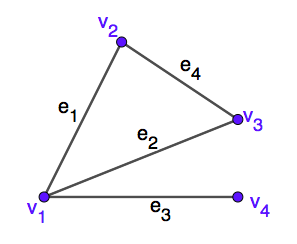
\includegraphics[scale=0.5]{fig/img/simpel_graf.png}
\caption{En simpel graf}
\label{fig:simpel}
\end{figure}
I kontrast til den simple graf finder vi multi-grafen. For denne type graf skal der være flere kanter, der forbinder det samme sæt punkter. Der må stadig ikke optræde løkker.
\begin{figure}[H]
\centering
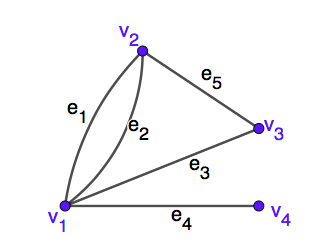
\includegraphics[scale=0.5]{fig/img/multigraf.png} 
\caption{En multigraf}
\label{fig:multi}
\end{figure}
I eksemplet ovenover ses det, at to kanter forbinder punktsættet ($v_{1},v_{2}$). Hvis en graf, modsat de to allerede nævnte, kan indeholde både løkker og flere kanter, der forbinder de samme punkter, kaldes det en pseudo-graf. Vi ser i eksemplet herunder, at der er to kanter, der forbinder $v_{1}$ og $v_{2}$, og der er en løkke ved $v_{4}$.
\begin{figure}[H]
\centering
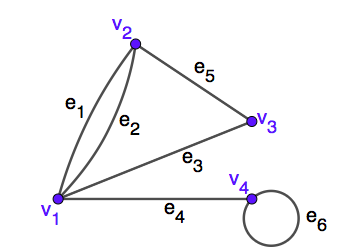
\includegraphics[scale=0.5]{fig/img/pseudograf.png}
\caption{En pseudograf med et loop}
\label{fig:pseudo}
\end{figure}
En anden grafopdeling man kan 
\subsection{Orienterede grafer og ikke-orienterede grafer}
En anden typisk grafopdeling er opdelingen i orienterede og ikke-orienterede grafer. De grafer vi har kigget på indtil videre er ikke-orienterede grafer. For en orienteret graf gælder det, at dets kanter har en retning. Dette er ofte illustreret med pile. Den har dermed et startpunkt og et endepunkt. Disse grafer er defineret ved:
\begin{definition}
[Orienteret graf] 
En orienteret graf $(V,E)$ består af $V$, et sæt punkter(knuder), hvor $V\neq0$, og et sæt orienterede kanter, $E$. Hver orienterede kant forbinder et sæt punkter $(u,v)$, hvor $u$ er tilstødende til $v$, og $v$ er tilstødende fra $u$. Punktet $u$ kaldes begyndelsespunktet, og punktet $v$ kaldes endepunktet.
\end{definition}
\begin{figure}[H]
\centering
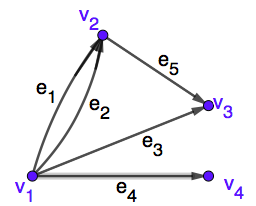
\includegraphics[scale=0.5]{fig/img/orienteret_graf.png}
\caption{En orienteret graf}
\label{fig:orienteret}
\end{figure}
Der kan foruden disse to også være tale om mixede grafer, som er grafer med både orienterede og ikke-orienterede kanter. Orienterede grafer kan ligesom ikke-orienterede grafer indeholde loops og flere kanter der forbinder det samme punktsæt. Den må også indeholde to modsatrettede kanter mellem det samme punktpar. Dvs. en kant må gerne gå fra $v$ til $u$, selvom en anden kant går fra $u$ til $v$. Hvis en orienteret graf hverken indeholder loops eller flere kanter, der forbinder det samme punktpar, kaldes den en orienteret simpel graf. Hvis der derimod optræder flere kanter mellem et eller flere punktpar, kaldes det en multigraf.Vi kan se egenskaberne for de forskellige grafer herunder:

\begin{tabular}{ |p{4cm}||p{3cm}|p{3cm}|p{2cm}|  }
 \hline
 \multicolumn{4}{|c|}{Grafer} \\
 \hline
 Type & Kanter & Flere Kanter pr punktpar tilladt? & Løkker tilladt\\
 \hline
 Simpel graf   & Ikke-orienteret    & Nej &   Nej\\
 Multigraf &   Ikke-orienteret & Ja   & Nej\\
 Pseudograf & Ikke-orienteret & Ja &  Ja\\
 Simpel orienteret graf    & Orienteret & Nej &  Nej\\
 Orienteret multigraf &  Orienteret  & Ja & Ja\\
 Mixet graf & Ikke-orienteret og orienteret  & Ja   & Ja\\
 \hline
\end{tabular}

Fordi kanterne i grafer med orienterede kanter er ordnede par kan definitionen af punktets grader være antallet af kanter, der har dette punkt som begyndelsespunkt, eller antallet af kanter, der har dette punkt som endepunkt:
\begin{definition}
[Graden af en orienteret graf] 
I en graf med orienterede kanter er ind-graden, betegnet ved $deg^{-}(v)$, antallet af kanter med v som deres endepunkt. Ud-graden, betegnet ved $deg^{+}(v)$, er antallet af kanter med v som deres startpunkt.
\end{definition}
Vi vil i projektet beskæftige os med orienterede grafer, da det er denne type vi bruger til optimeringen af gaslageret. I vores tilfælde vil vi tildele vores orienterede kanter vægt, hvilket beskrives senere i projektet.

\input{incl/main/grafer/repræsentation}
\subsection{Nabolister}
En måde at repræsentere en graf på er ved at lave en naboliste. Nabolister er tabeller, der giver en oversigt over hvilke knuder, der er forbundet med andre knuder. Dog vil man ikke kunne se, hvis der er parallelle kanter. En naboliste er bygget op således, at knuden, man vil beskrive, er i venstre side af tabellen, og naboknuderne er skrevet i højre side. \\

\begin{figure}[h]
  \centering
  \begin{tikzpicture}
    \node[point] at (1,2) (A) [label=above:\(A\)] {};
    \node[point] at (3,2) (B) [label=above:\(B\)] {};
    \node[point] at (4,1) (C) [label=right:\(C\)] {};
    \node[point] at (2,0) (D) [label=below:\(D\)] {};
    \node[point] at (3,0) (E) [label=below:\(E\)] {};
    \node[point] at (1,1) (F) [label=left:\(F\)] {};
    \node[point] at (0,2) (G) [label=below:\(G\)] {};

    \footnotesize
    \draw (A) -- (G);
    \path (F) edge [bend left] (B);
    \draw (A) -- (F);
    \path (F) edge [bend right] (B);
    \draw (B) -- (D);
    \draw (B) -- (E);
    \draw (B) -- (C);
    \draw (C) -- (E);
    \draw (C) to [out=315,in=45,looseness=50] (C);
    \draw (E) -- (D);
    \draw (D) -- (F);
    \draw (F) -- (G);
  \end{tikzpicture}
  \caption{Ikke-orienteret pseudograf.}
  \label{fig:ikke-orienteret-pseudo}
\end{figure}

\begin{center}
	\begin{tabular}{ |p{4cm}||p{3cm}|}
	 	\hline
 		\multicolumn{2}{|c|}{Naboliste til figur \ref{fig:ikke-orienteret-pseudo}} \\
 		\hline
 		Knuder & Naboknuder\\
 		\hline
 		A & F,G \\
		B & C,D,E,F \\
		C & B,E,C \\
		D & B,E,F \\
		E & B,C,D \\
		F & A,B,D,G \\
		G & A,F \\
 	\hline
 	\label{tab:naboliste} 	
	\end{tabular}
	%\caption{Naboliste til figur \ref{fig:ikke-orienteret-pseudo}
\end{center}
Ud fra tabellen ses, at knuden B har naboknuderne C, D, E og F, men man kan ikke se, at der er en ekstra kant mellem B og F. Dog kan man se, at C har en løkke, da den er nabo til sig selv.

\begin{figure}[H]
  \centering
  \begin{tikzpicture}
    \node[point] at (1,2) (A) [label=above:\(A\)] {};
    \node[point] at (3,2) (B) [label=above:\(B\)] {};
    \node[point] at (4,1) (C) [label=right:\(C\)] {};
    \node[point] at (2,0) (D) [label=below:\(D\)] {};
    \node[point] at (3,0) (E) [label=below:\(E\)] {};
    \node[point] at (1,1) (F) [label=left:\(F\)] {};
    \node[point] at (0,2) (G) [label=below:\(G\)] {};

    \footnotesize
    \path [->] (A) edge [bend left] (G);
    \path [->] (A) edge [bend right] (G); 
    \path [->] (F) edge [bend left] (B);
    \draw [<-](A) -- (F);
    \path [<-](F) edge [bend right] (B);
    \draw [->](B) -- (D);
    \draw [<-](B) -- (E);
    \draw [<-](B) -- (C);
    \draw [->](C) -- (E);
    \draw [->](C) to [out=315,in=45,looseness=50] (C);
    \draw [<-](E) -- (D);
    \draw [->](D) -- (F);
    \draw [->](F) -- (G);
  \end{tikzpicture}
  \caption{Orienteret pseudograf.}
  \label{fig:orienteret-pseudo}
\end{figure}

%\begin{center}
%	\begin{tabular}{ |p{4cm}||p{3cm}|}
%	 	\hline
% 		\multicolumn{2}{|c|}{Naboliste til figur \ref{fig:orienteret-pseudo} \\
% 		\hline
% 		Knuder & Naboknuder\\
% 		\hline
% 		A & G \\
%		B & D,F \\
%		C & B,E,C \\
%		D & E,F \\
%		E & B \\
%		F & A,B,G \\
%		G &  \\
% 	\hline
% 	\label{tab:naboliste1}
%	\end{tabular}
%\end{center}

\ref{tab:naboliste1} viser en oversigt over den orienterede grafs (Figur \ref{fig:orienteret-pseudo}) naboknuder. Kigger man på B og F i tabellen, kan man se, at der er parallelle kanter, da kanterne er orienteret i hver deres retning. Kigger man på A og G, kan man ikke se, at der er parallelle kanter mellem A og G, da begge kanter er orienteret fra A til G.
\subsection{Nabomatricer}
En anden mulighed for at repræsentere en graf er ved brug af nabomatricer. Nabomatricer er bedre, når grafen har mange kanter.\\
En nabomatrice kan beskrives som en $N=m X m$ matrice, hvor $m$ er afhængig af knudemængden $V=\{v_0, v_1, \ldots, v_m\}$. Hvis man har en simpel graf, $G=(V,E)$, vil matricen være en nul-1 matrice, da en simpel graf kan kun have en kant mellem to knuder. Når der er en kant mellem to  vilkårlig knuder, $(v_i,v_j)$,  vil den få notationen 1, hvis der derimod ikke er en kant vil får den notation 0. \\

Det kan også skrives som \\

\begin{equation}
\begin{Bmatrix} 
	 \hspace{0.3cm}\textrm{1 hvis} \hspace{0.3cm}\{v_i,v_j\} \hspace{0.2cm} \textrm{har en kant i grafen} \hspace{0.2cm} G \\
	 \textrm{0 ellers} \\
	\end{Bmatrix}
\end{equation}

\begin{figure}[H]
  \centering
  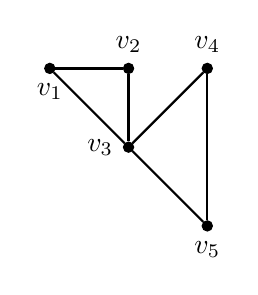
\begin{tikzpicture}
  \tikzset{enclosed/.style={draw, circle, inner sep=0pt, minimum size=.13cm, fill=black}}
  	\node[enclosed] at (0,2) (v1) [label=below:\(v_1\)] {};
    \node[enclosed] at (1,2) (v2) [label=above:\(v_2\)] {};
    \node[enclosed] at (1,1) (v3) [label=left:\(v_3\)] {};
    \node[enclosed] at (2,2) (v4) [label=above:\(v_4\)] {};
    \node[enclosed] at (2,0) (v5) [label=below:\(v_5\)] {};
    
	\path[thick] (v1) edge node {} (v2);
	\path[thick] (v1) edge node {} (v3);
	\path[thick] (v2) edge node {} (v3);
	\path[thick] (v4) edge node {} (v3);
	\path[thick] (v5) edge node {} (v3);   
	\path[thick] (v4) edge node {} (v5); 

  \end{tikzpicture}
  \caption{Ikke-orienteret, simpel graf.}
  \label{fig:stm}
\end{figure}

  \label{fig:simpelgraf}
\end{figure}

Nabo natricen nedenfor bruger rækkefølgen $v_1$,$v_2$,$v_3$,$v_4$,$v_5$
\begin{equation}
	\begin{bmatrix}
		0&1&1&0&0 \\
		1&0&1&0&0 \\
		1&1&0&1&1 \\
		0&0&1&0&1 \\
		0&0&1&1&0 \\
	\end{bmatrix}
\end{equation}

	



\section{Veje}
Vi har indtil videre snakket om kanter, og hvordan de enkeltvis er incidente med knudepar. I dette afsnit vil vi udvide det til at snakke om veje, som er følger af disse kanter, og dermed er de også grafer i sig selv. Hvis der er tale om ikke-orienterede grafer, er veje defineret ved:
\begin{defn}
[Veje i ikke-orienterede grafer] 
Lad $n \in \N _0$  og $G$ være en ikke-orienteret graf. En vej, $P$, af længde $n$, fra $u$ til $v$, i $G$ er en følge af $n$ kanter,  $ P= (e_{1},e_{2},\dotsc,e_{n})$, for hvilken der eksisterer en følge, $u=x_{0}$ og $v=(x_{1},x_{2},\dotsc,x_{n-1}$,$x_{n})$, af knuder sådan at $e_{i}$ har, for $i=1,2,\dotsc,n$, endeknuderne $x_{i-1}$ og $x_{i}$. Når grafen er simpel, betegnes vejen ved grafens knudefølge, $x_{o},x_{1},\dotsc,x_{n}$. Hvis den ikke er simpel, beskrives vejen ved kanterne, $e_{1},e_{2},\dotsc,e_{n}$. 
\end{defn}
Her er en vej simpel, hvis den kun passerer den samme kant én gang. Kigger vi derimod på veje med orienterede grafer, som er det vi beskæftiger os med i problemet, ser definitionen en smule anderledes ud:
\begin{defn}
[Veje i orienterede grafer] 
Lad $n \in \N _0$ og $G$ være en orienteret graf. En vej, $P$, af længde $n$, fra $u = x_0$ til $v = x_n$, i $G$ er en følge af kanter, $e_{1},e_{2},\dotsc,e_{n}$, $ \exists (x_{n-1},x_{n}) $ for $e_{n} \forall e_n$. Hvis alle knudepar, i en given vej, højst har én kant som er incident med parret, betegner vi vejen ved dennes knudefølge $x_{o},x_{1},\dotsc,x_{n}$.
\end{defn}

\begin{figure}[H]
\centering
	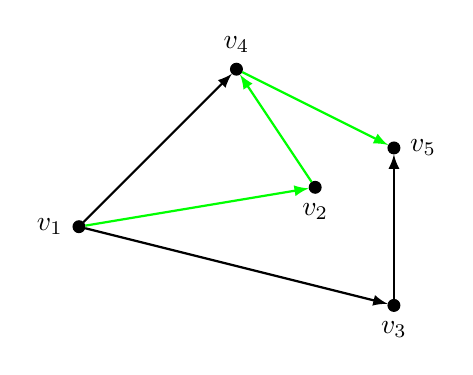
\begin{tikzpicture}

      \tikzset{enclosed/.style={draw, circle, inner sep=0pt, minimum size=.15cm, fill=black}}
%% Vertices
      	\node[enclosed, label={left: $v_1$}] (v1) at (0,2) {};
      	\node[enclosed, label={below: $v_2$}] (v2) at (3,2.5) {};
    		\node[enclosed, label={below: $v_3$}] (v3) at (4,1) {};
  	    \node[enclosed, label={above: $v_4$}] (v4) at (2,4) {};
     	\node[enclosed, label={right: $v_5$}] (v5) at (4,3) {};
%Edges
		\path [->, >=latex, thick, green](v1) edge node[midway, sloped, above] {} (v2);
		\path [->, >=latex, thick](v1) edge node[midway, sloped, above] {} (v3);
		\path [->, >=latex, thick](v1) edge node[midway, above] {} (v4);
		\path [->, >=latex, thick, green](v2) edge node[near end, sloped, below] {} (v4);
		\path [->, >=latex, thick](v3) edge node[midway, below] {} (v5);
		\path [->, >=latex, thick, green](v4) edge node[near end, sloped, above] {} (v5);

	\end{tikzpicture}
	\caption{Eksempel på en orienteret simpel graf og en vej fra $v_{0}$ til $v_{4}$}
	\label{fig.vaegtetopg}
\end{figure}

Antallet af veje mellem to knuder i grafen kan findes ved hjælp af nabomatricer, som vi diskuterede i forrige afsnit.
\begin{thm}
[Antallet af veje mellem to knuder] 
Lad G være en vilkårlig graf med nabomatricen
\textbf{$A$} med grafens knuder i rækkefølgen $v_{1},v_{2},\dotsc,v_{n}$. Antallet af forskellige veje med længde $r$ fra $v_{i}$ til $v_{j}$ vil da være lig den $(i,j)$'te indgang af \textbf{$A^{r}$}.
\end{thm}

\begin{proof}
Bevis: Lad G være en graf med nabomatricen 
\textbf{$A$}, hvor vi antager, at knuderne i $G$ har rækkefølgen $v_{1},v_{2},\cdots,v_{n}$. Antallet af veje fra $v_{i}$ til $v_{j}$ af længde 1 er da den $(i,j)$'te indgang til 
\textbf{$A$}. Dette skyldes, at det blot er antallet af kanter fra $v_{i}$ til $v_{j}$.
Vi antager, at den $(i,j)$'te indgang til 
\textbf{${A^r}$} er antallet af forskellige veje, som går fra $v_{i}$ til $v_{j}$ og som har længden $r$. Dette er hypotesen, vi ønsker at bekræfte.
Vi ser på nabomatricen \textbf{$A^{r+1}$}. 
\textbf{$A^{r+1}$} er det samme som 
\textbf{$A^{r}$}$\dotsc$\textbf{$A$}, og derfor er den $(i,j)$'te indgang af \textbf{$A^{r+1}$} lig med $b_{i1}a_{1j} + b_{i2}a_{2j} +\dotsc+ b_{in}a_{nj}$. Her er $b_{ik}$  den $(i,k)$'te indgang til 
\textbf{$A^{r}$}, som ifølge vores hypotese er antallet af veje fra $v_{i}$ til $v_{k}$ med længde $r$.
En vej af længde $r + 1$ fra $v_{i}$ til $v_{k}$ er lavet ud fra en vej med længden $r$ fra begyndelsesknuden $v_{i}$ og hen til en mellemliggende knude $v_{k}$ samt den kant, der går fra $v_{k}$ til $v_{j}$. Vi ved fra kombinatorik, at antallet af muligheder er lig produktet af mulighederne ved første udfald og mulighederne ved andet udfald. Vi betegner antallet af veje med længden $r$ fra $v_{i}$ til $v_{k}$ med $b_{ik}$ og antallet af kanter fra $v_{k}$ til $v_{j}$ med $a_{kj}$ Finder vi produktet af dette for alle mellemliggende knuder, $v_{k}$, fås det ønskede resultat.
\end{proof}

\begin{exmp}
Vi starter med at kigge på en graf og den tilhørende nabomatrice:
\begin{figure}[H]
\centering
	\begin{tikzpicture}

      \tikzset{enclosed/.style={draw, circle, inner sep=0pt, minimum size=.15cm, fill=black}}
%% Vertices
      	\node[enclosed, label={left: $v_1$}] (v1) at (1,2) {};
      	\node[enclosed, label={above: $v_2$}] (v2) at (3,4) {};
    	\node[enclosed, label={below: $v_3$}] (v3) at (1,0) {};
  	    \node[enclosed, label={right: $v_4$}] (v4) at (5,2) {};
     	\node[enclosed, label={below: $v_5$}] (v5) at (5,0) {};
%Edges
		\path (v1) edge node[midway, sloped, above] {} (v2);
		\path (v1) edge node[midway, sloped, above] {} (v3);
		\path (v1) edge node[midway, above] {} (v4);
		\path (v2) edge node[near end, sloped, below] {} (v4);
		\path (v3) edge node[midway, below] {} (v5);
		\path (v4) edge node[near end, sloped, above] {} (v5);

	\end{tikzpicture}
	\caption{Eksempel på en ikke-orienteret simpel graf}
	\label{fig.vaegtetopg}
\end{figure}

\begin{equation}
A=\begin{bmatrix}
    0&1&1&1&0\\
    1&0&0&1&0\\
    1&0&0&0&1\\
    1&1&0&0&1\\
    0&0&1&1&0\\
\end{bmatrix}
\end{equation}


Vi ønsker at finde ud af hvor mange veje med en længde på 4, der går fra $v_1$ til $v_5$. Det ses i nabomatricen, at $v_1$ har 3 naboer, nemlig $v_2$, $v_3$ og $v_4$. Fortsætter vi, kan vi se, at $v_2$ har $v_1$ og $v_4$ som naboer, $v_3$ har $v_1$ og $v_5$, og $v_4$ har $v_1$, $v_2$ og $v_5$ som naboer. Fortsætter vi, så vi finder alle tænkelige veje med længder på 3, får vi, at der er 18 forskellige veje, der alle starter i $v_1$ og har en længde på 3. Vi skal nu finde de veje, der ved at tilføje en kant, ender i $v_5$. Vi kan se, at $v_5$ har $v_3$ og $v_4$ som naboer. Vi finder derfor de veje, der starter i $v_1$ og slutter i $v_3$, med længden 3, og derefter dem, der slutter i $v_4$, med længden 3. På denne måde udnytter vi, hvad vi skrev i beviset, nemlig at
\textbf{$A^{r+1}$} er lig med $b_{i1}a_{1j} + b_{i2}a_{2j} +\cdots+ b_{in}a_{nj}$
Her er $b_{ik}$ antallet af veje fra $v_{i}$ til ${v_k}$. I vores eksempel er $v_{i}=v_{1}$, ${v_{k1}}=v_{3}$, ${v_{k2}}=v_{4}$, $v_{j}=v_{5}$ og \textbf{$A^{r+1}$}=\textbf{$A^{3+1}$}. 
 
\begin{figure}[H]
\centering
	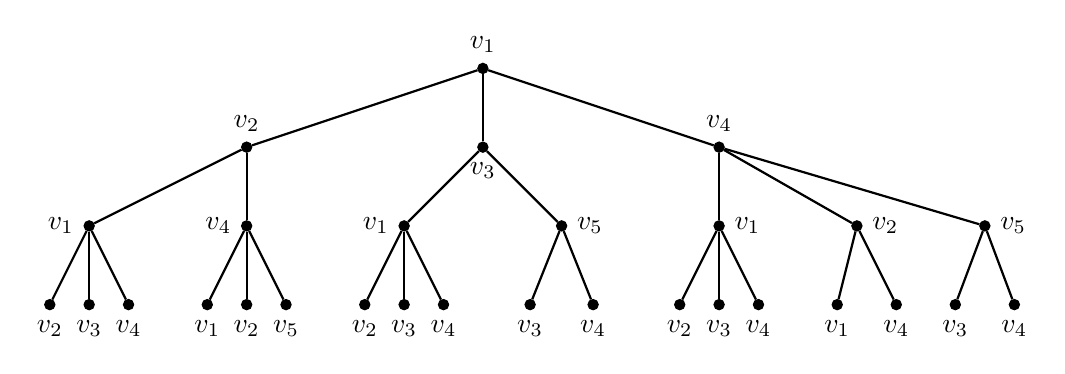
\begin{tikzpicture}

      \tikzset{enclosed/.style={draw, circle, inner sep=0pt, minimum size=.13cm, fill=black}}
%% Vertices
      	\node[enclosed, label={above: $v_1$}] (v1) at (3,6) {};
      	\node[enclosed, label={above: $v_2$}] (v2) at (0,5) {};
    		\node[enclosed, label={below: $v_3$}] (v3) at (3,5) {};
  	    \node[enclosed, label={above: $v_4$}] (v4) at (6,5) {};
     	\node[enclosed, label={left: $v_1$}] (v5) at (-2,4) {};
     	\node[enclosed, label={left: $v_4$}] (v6) at (0,4) {};
     	\node[enclosed, label={left: $v_1$}] (v7) at (2,4) {};
     	\node[enclosed, label={right: $v_5$}] (v8) at (4,4) {};
     	\node[enclosed, label={right: $v_1$}] (v9) at (6,4) {};
     	\node[enclosed, label={right: $v_2$}] (v10) at (7.75,4) {};
     	\node[enclosed, label={right: $v_5$}] (v11) at (9.375,4) {};
     	\node[enclosed, label={below: $v_2$}] (v12) at (-2.5,3) {};
      	\node[enclosed, label={below: $v_3$}] (v13) at (-2,3) {};
  	    \node[enclosed, label={below: $v_4$}] (v14) at (-1.5,3) {};
  	    \node[enclosed, label={below: $v_1$}] (v15) at (-0.5,3) {};
     	\node[enclosed, label={below: $v_2$}] (v16) at (0,3) {};
     	\node[enclosed, label={below: $v_5$}] (v17) at (0.5,3) {};
     	\node[enclosed, label={below: $v_2$}] (v18) at (1.5,3) {};
      	\node[enclosed, label={below: $v_3$}] (v19) at (2,3) {};
  	    \node[enclosed, label={below: $v_4$}] (v20) at (2.5,3) {};
  	    \node[enclosed, label={below: $v_3$}] (v21) at (3.6,3) {};
  	    \node[enclosed, label={below: $v_4$}] (v22) at (4.4,3) {};
  	    \node[enclosed, label={below: $v_2$}] (v23) at (5.5,3) {};
      	\node[enclosed, label={below: $v_3$}] (v24) at (6,3) {};
  	    \node[enclosed, label={below: $v_4$}] (v25) at (6.5,3) {};
  	    \node[enclosed, label={below: $v_1$}] (v26) at (7.5,3) {};
     	\node[enclosed, label={below: $v_4$}] (v27) at (8.25,3) {};
     	\node[enclosed, label={below: $v_3$}] (v28) at (9,3) {};
     	\node[enclosed, label={below: $v_4$}] (v29) at (9.75,3) {};
%Edges
		\path[thick] (v1) edge node[midway, sloped, above] {} (v2);
		\path[thick] (v1) edge node[midway, sloped, above] {} (v3);
		\path[thick] (v1) edge node[midway, above] {} (v4);
		\path[thick] (v2) edge node[near end, sloped, below] {} (v5);
		\path[thick] (v2) edge node[midway, below] {} (v6);
		\path[thick] (v3) edge node[near end, sloped, above] {} (v7);
		\path[thick] (v3) edge node[near end, sloped, above] {} (v8);
		\path[thick] (v4) edge node[near end, sloped, above] {} (v9);
		\path[thick] (v4) edge node[near end, sloped, above] {} (v10);
		\path[thick] (v4) edge node[near end, sloped, above] {} (v11);
		\path[thick] (v5) edge node[near end, sloped, above] {} (v12);
		\path[thick] (v5) edge node[near end, sloped, above] {} (v13);
		\path[thick] (v5) edge node[near end, sloped, above] {} (v14);
		\path[thick] (v6) edge node[near end, sloped, above] {} (v15);
		\path[thick] (v6) edge node[near end, sloped, above] {} (v16);
		\path[thick] (v6) edge node[near end, sloped, above] {} (v17);
		\path[thick] (v7) edge node[near end, sloped, above] {} (v18);
		\path[thick] (v7) edge node[near end, sloped, above] {} (v19);
		\path[thick] (v7) edge node[near end, sloped, above] {} (v20);
		\path[thick] (v8) edge node[near end, sloped, above] {} (v21);
		\path[thick] (v8) edge node[near end, sloped, above] {} (v22);
		\path[thick] (v9) edge node[near end, sloped, above] {} (v23);
		\path[thick] (v9) edge node[near end, sloped, above] {} (v24);
		\path[thick] (v9) edge node[near end, sloped, above] {} (v25);
		\path[thick] (v10) edge node[near end, sloped, above] {} (v26);
		\path[thick] (v10) edge node[near end, sloped, above] {} (v27);
		\path[thick] (v11) edge node[near end, sloped, above] {} (v28);
		\path[thick] (v11) edge node[near end, sloped, above] {} (v29);

	\end{tikzpicture}
	\caption{De mulige løsninger for veje med længde 3 fra $v_{0}$ til $v_{k}$.}
	\label{fig.vaegtetopg}
\end{figure}

Antallet af veje fra $v_{1}$ til $v_{3}$ er 5, og antallet af veje fra $v_{1}$ til $v_{4}$ er 6. Vi kan derfor opstille
\textbf{$A^{4}$}$=b_{i1} a_{1j}+b_{i2} a_{2j}=5 \cdot 1+6 \cdot 1=11$.
Her er $b_{i1}$ antallet af veje fra $v_{1}$ til $v_{3}$, og $a_{1j}$ er antallet af kanter fra $v_{3}$ til  $v_{5}$. På samme måde optræder $b_{i2}$ og $a_{2j}$ for $v_{4}$. Der er altså 11 veje med længden 4 fra $v_{1}$ til $v_{5}$.

\end{exmp}

\input{incl/main/grafer/vægtede}

\section{Delte grafer}
I visse tilfælde kan en graf deles op, for at optimere en algoritme til løsningen af problemet i en given problemstilling. \\
To måder at dele en graf op er $k$-delte grafer og delgrafer.

\begin{defn} \label{defn:k-delt} %k-partite
En graf G kaldes en $k$-delt graf $G = (V_1, V_2, \ldots, V_k; E)$, hvis følgende betingelser opfyldes: $V= V_i \cup V_j, V_i \cap V_j = Ø \forall i,j$, og $i\neq j$ 
\end{defn}

En $k$-delt graf består af $k$ disjunkte, ikke-tomme delmængder, $V_1, V_2, \ldots, V_k$, hvor for 2 vilkårlige knuder, $u$ og $v$, kun er forbundet, hvis de er i forskellige delmængder.
\begin{defn}	 \label{defn:delgraf} %subgraph
En delgraf af grafen $G= (V,E)$ er en graf $D = (W,F)$ skabt af delelementerne af kanterne og knuderne: $W \subseteq V og F \subseteq E$.
\end{defn}

Fordelen ved at dele en graf op i forskellige delgrafer er, at når man i $korteste-vej$, eller i bestemte tilfælde $længste-vej$, kan finde den optimale delstruktur hvis den optimale delgraf er fundet. Altså finder man den optimale vej igennem knuderne $(a, c, g, n)$, er den optimale vej også fundet til de mellemliggende knuder også fundet, altså fra $a$ til fx $g$.







\chapter{Analyse}
\section{Sektion 1}

\section{Sektion 2}

\section{Sektion 3}


\chapter{Vurdering af metoderne}
\section{Sektion 1}

\section{Sektion 2}

\section{Sektion 3}

\chapter{Konklusion}
Procesoptimering er en vigtige del af, hvordan virksomheder øger deres profit. Dette gælder også for ejere af gaslagre, som ved at købe og sælge gas skal forsøge at balancere mellem at være konkurrencedygtige på markedet med fornuftige priser og samtidig tjene mest muligt. Denne balance har vi forsøgt at finde ved at arbejde med grafteori og algoritmer. På baggrund af teorien bag disse emner har vi opstillet en graf for et gaslagers mulige køb og salg i løbet af det år vi lejer lageret. 

Derudover har vi udarbejdet en algoritme i programmet Python 3, som kan opstimere handelsstrategien for gaslageret ved at finde den vej gennem den omtalte graf, der giver den største profit. For vores basisproblem gælder det, at den maksimale profit ud fra de givne værdier i opgaven er 252,72 euro. Denne opnås ved at følge handelsstrategierne givet i (Figur ?). Dette er også illustreret på (Graf ?) 

Vores algoritme kan med få ændringer tilpasses så den også kan anvendes på vores udvidede problem. I vores udvidede problem skal vi tage højde for at lageret ikke har faste grænseværdier, men minimums- og maksimumsindholdet svinger alt efter, hvilken måned vi befinder os i. På samme måde ændrer antallet af gasenheder, som vi må købe og sælge, sig. Derudover er der i det udvidede problem også en straffaktor, hvis lagerbeholdningen til sidst ikke er $q_goal$. Dette betyder at gaslagerets ejer ikke vil købe gassen tilbage for fuld pris, hvis ikke vi har ramt $q_goal$. Den største profit, som vi kunne få med det udvidede problem var 188,27 euro. Denne opnås ved at følge handelsstrategien givet i (Figur ?). Dette er også illustreret på (Graf ?)


Det ses altså, at udvidelserne mindsker profitten betragteligt, og især de svingende grænser for $q_max$, $q_min$, $u_max$ og $i_max$ har betydning, da de påvirker profitten over flere måneder og ikke kun i den sidste måned, som straffaktoren gør. Hvis man ønsker at maksimere sin profit, skal man derfor forsøge at mindske nogle af disse udvidelser, hvis dette er muligt.



%\chapter{Forord}
Følgende projekt er udarbejdet af gruppe B350 bestående af fem stud.scient.oeconer på 1. semester. Projektet er skrevet i efteråret 2020 og beskæftiger sig med diskret matematik herunder optimering af et gaslager som basisproblem. Diskret matematik indgår i studiets læreplan og er derfor et relevant emne til projektskrivning. Projektet er skrevet i \LaTeX, og delt via GitAhead.
%Vi vil som gruppe rette en stor tak til vores vejleder Janus Valberg-Madsen for godt samarbejde gennem projektforløbet samt gode råd og rettelser.







% Input-filer bør opdeles således, at hver fil svarer til et kapitel. Makroen
% \include indsætter et sideskift og indholdet fra den givne stil.

% \include{incl/main/example1}
% \include{incl/main/example2}
% ...

% Appendicer indsættes inde i en appendices-blok og bliver nummereret med
% bogstaver i stedet for tal
\begin{appendices}
  % \include{incl/app/appendix1}
  % \include{incl/app/appendix2}
  % ..
\end{appendices}

% Dokumentets 'back matter' er til ekstra ting som f.eks. litteraturlisten.
% Overskrifter bliver ikke nummereret her.
\backmatter

% Automatisk litteraturliste baseret på, hvilke kilder, der er blevet refereret
% til i løbet af rapporten.
\bibliographystyle{apalike}
\bibliography{
  incl/bib/books,
  incl/bib/articles,
  incl/bib/software
}
\end{document}
